\documentclass[12pt, a4paper]{article}

\usepackage{amsmath}
\usepackage{array}
\usepackage{amsmath}
\usepackage[portuguese]{babel}
\usepackage{chngpage}
\usepackage{float}
\usepackage[a4paper, margin=2cm]{geometry}
\usepackage{graphicx}
\usepackage{hyperref}
\usepackage{listings}
\usepackage{setspace}
\usepackage{xcolor}

\lstdefinestyle{codestyle}{
    commentstyle=\color{teal},
    keywordstyle=\color{blue},
    numberstyle=\ttfamily\color{gray},
    stringstyle=\color{red},
    basicstyle=\ttfamily\footnotesize,
    breakatwhitespace=false,
    breaklines=false,
    keepspaces=true,
    numbers=none,
    showspaces=false,
    showstringspaces=false,
    showtabs=false,
    tabsize=4
}
\lstset{style=codestyle}

\title{\Huge \textbf{Computação Gráfica \\ \Large Trabalho Prático -- Fase II}}
\date{30 de março 2025}
\author{Grupo 3}

\begin{document}

\begin{center}
    
\includegraphics[width=0.25\textwidth]{res/cover/EE-C.eps}
\end{center}

\chardef\_=`_
\onehalfspacing
\setlength{\parskip}{\baselineskip}
\setlength{\parindent}{0pt}
\def\arraystretch{1.5}

{\let\newpage\relax\maketitle}
\maketitle
\thispagestyle{empty}

\vspace*{\fill}

\begin{adjustwidth}{-2cm}{-2cm} % These values only need to be large enough to center the table
    \begin{center}
        \begin{tabular}{>{\centering}p{0.25\textwidth}
                        >{\centering}p{0.25\textwidth}
                        >{\centering}p{0.25\textwidth}
                        >{\centering\arraybackslash}p{0.25\textwidth}}
            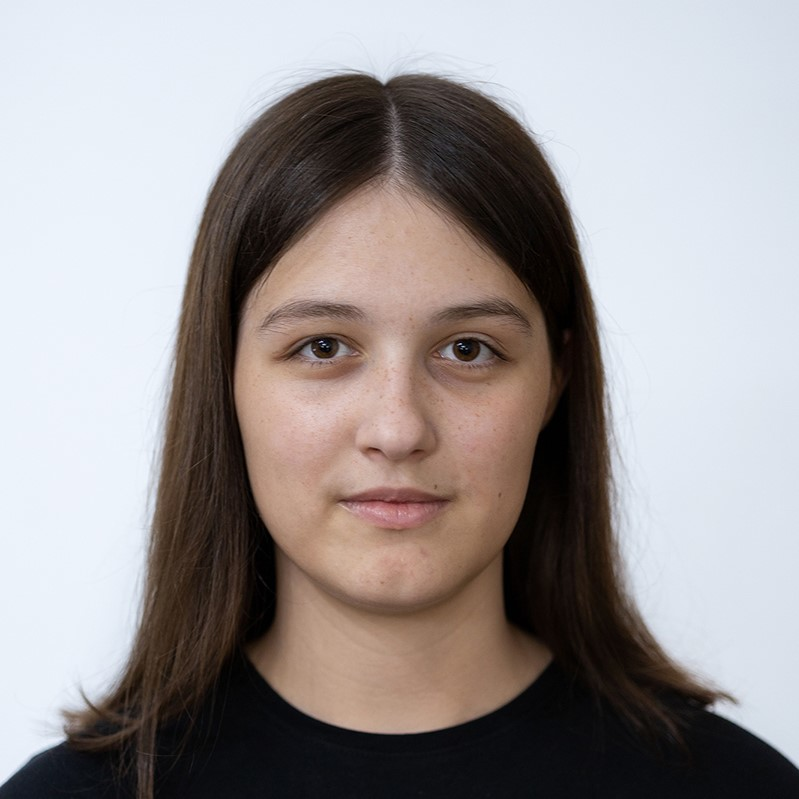
\includegraphics[width=3.5cm]{res/cover/A104437.png} &
            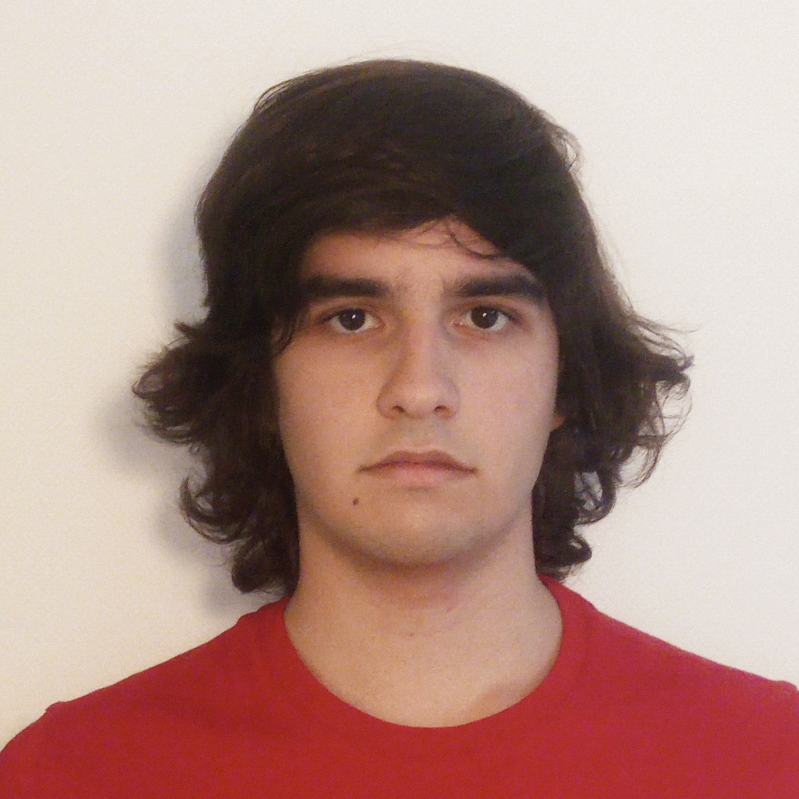
\includegraphics[width=3.5cm]{res/cover/A104348.png} &
            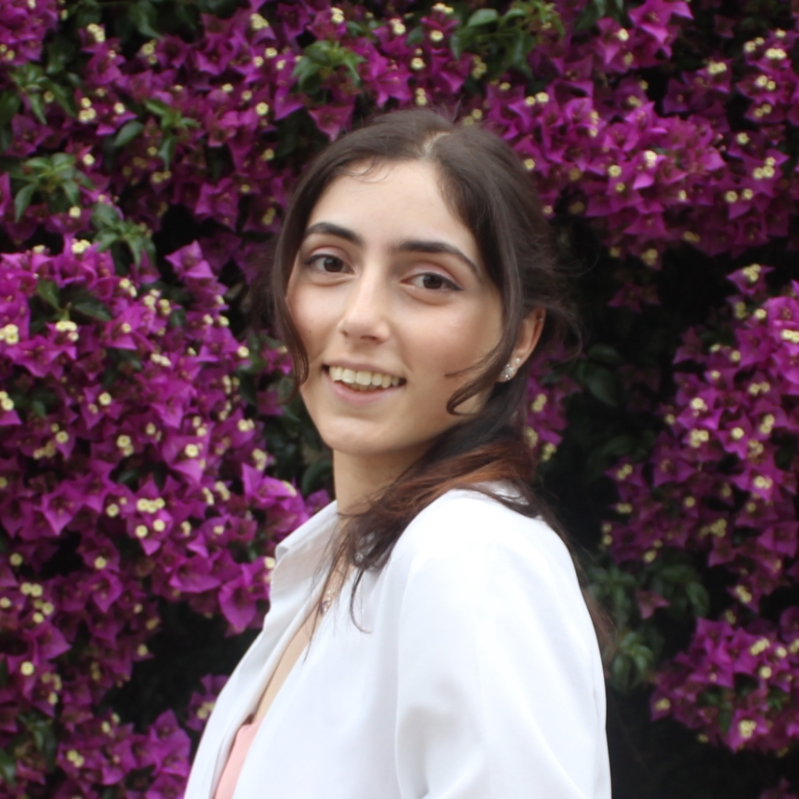
\includegraphics[width=3.5cm]{res/cover/A90817.png} &
            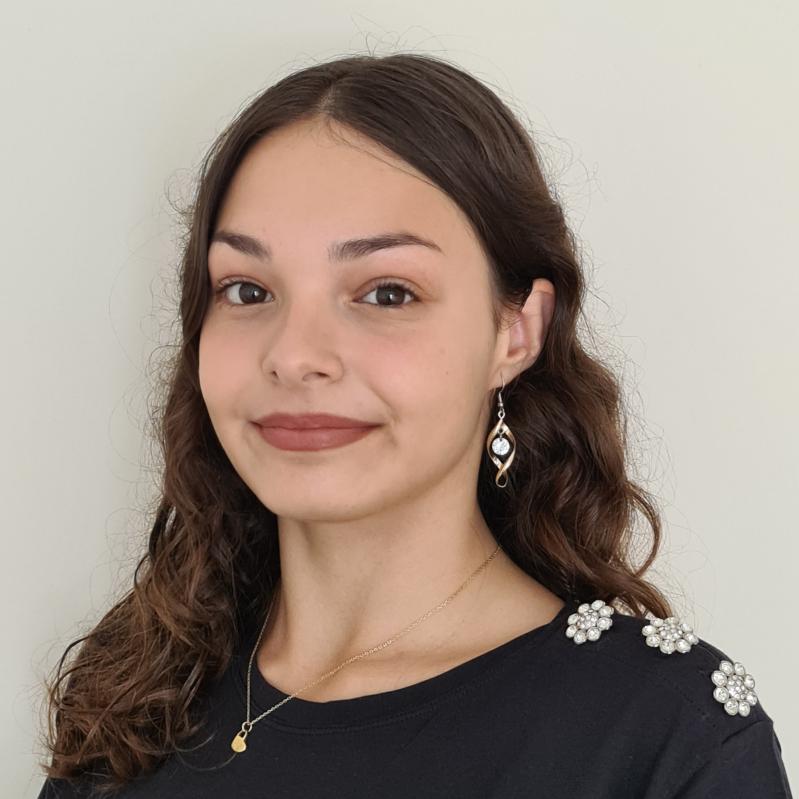
\includegraphics[width=3.5cm]{res/cover/A104179.png} \\

            Ana Oliveira & Humberto Gomes & Mariana Cristino & Sara Lopes \\
            A104437      & A104348        & A90817           & A104179
        \end{tabular}
    \end{center}
\end{adjustwidth}

\pagebreak

\begin{abstract}
    \textbf{\color{red} TODO - resumo}
\end{abstract}

\section{Transformações}

\textbf{\color{red} TODO - transformações}

\section{Modelo estático do sistema solar}

\textbf{\color{red} TODO - sistema solar}

\section{Extras}

\subsection{Câmara Orbital}

A câmara orbital é uma câmara virtual que permite observar uma scene a partir de um ponto que
orbita à volta de um objeto ou de um ponto de vista (\texttt{lookAt}). Na implementação atual, este
ponto de interesse está fixado na origem do espaço tridimensional. Esta abordagem é útil para
observar um objeto de diversos ângulos possíveis com o foco num ponto em específico.

\subsubsection{Movimentação e Controlo}

A câmara orbital é definida por 3 parâmetros:
\begin{itemize}
    \item Raio (\texttt{radius}): determina a distância do ponto de interesse à câmara;
    \item Ângulo azimutal ($\phi$): define a rotação da câmara em torno do eixo vertical,
    o que permite uma visualização de 360 graus ao redor do objeto;
    \item Ângulo polar ($\theta$): controla o ângulo de elevação da câmara.
\end{itemize}

A atualização da a posição da câmara é dada pela soma do ponto de interesse (\texttt{lookAt}) com
as coordenadas cartesianas obtidas a partir das coordenadas esféricas. As fórmulas utilizadas para
a conversão são as seguintes:

$$x = radius \times \sin(\theta) \times \cos(\phi)$$
$$y = radius \times \cos(\theta)$$
$$z = radius \times \sin(\theta) \times \sin(\phi)$$

De forma a garantir um comportamento estável e consistente, os valores são restringidos a
intervalos pré-definidos. O raio encontra-se limitado entre $0.5$ e $100$, para evitar que a câmara
se aproxime demasiado ou se afaste demasiado do ponto de interesse. O ângulo azimutal varia entre
$0$ e $2\pi$, para que a rotação aconteça de forma contínua. Por fim, o ângulo polar encontra-se
entre $0.01$ e $\pi - 0.01$ para evitar que a câmara alcance os polos e cause instabilidade no
movimento, no sentido em que se $\theta$ atingir o valor $\pi$, o vetor \texttt{up} da câmara
ficaria invertido, de modo que a câmara viraria completamente ao contrário. Assim, os comandos
também ficariam invertidos, isso tornaria a navegação confusa e pouco intuitiva.

\subsubsection{Controlo pelo Utilizador}

Para controlar a câmara orbital, o utilizador utiliza o teclado, sendo que as teclas associadas a
cada ação são:
\begin{itemize}
    \item \texttt{W}: inclina a câmara para cima;
    \item \texttt{S}: inclina a câmara para baixo;
    \item \texttt{A}: roda a câmara para a esquerda;
    \item \texttt{D}: roda a câmara para a direita;
    \item \texttt{F}: aproxima a câmara do ponto de interesse;
    \item \texttt{B}: afasta a câmara do ponto de interesse.
\end{itemize}

\section{Resultados obtidos}

\textbf{\color{red} TODO - resultados}

\section{Conclusão e Trabalho Futuro}

\textbf{\color{red} TODO - conclusão}

\begingroup
\section{Bibliografia}
\renewcommand{\section}[2]{}

\begin{thebibliography}{9}
    \bibitem{exemplo}
        \href{https://youtu.be/dQw4w9WgXcQ}{Um item de exemplo na bibliografia}
\end{thebibliography}
\endgroup

\end{document}
